% Provenance (never printed): see sources/outline_sources.md (Year 1:
% geological cross-sections, apparent dip, thickness, boreholes). Every
% Varden Hills number comes from figdata/bachelor-1/varden_sections.py, which
% imports the shared model figdata/shared/region.py; numbers of the exercises
% and problem in the Book 3 scratch calculator and in that script's values.
\chapter{Penampang geologi}\label{ch:b1:cross-sections}

Sebuah perusahaan teknik merencanakan terowongan di bawah Perbukitan Varden, lurus dari barat ke timur pada ketinggian tetap \qty{200}{m}. Sebelum satu meter pun dibor, para ahli geologi harus menyatakan batuan apa yang akan dipotong mesin, di mana ia akan melintasi sesar, dan berapa lama ia akan berada di batu gamping, batuan yang mungkin menyimpan rongga terbuka dan air. Tidak seorang pun dapat melihat ke dalam bukit-bukit itu; tetapi \omterm{def:b1:geological-maps:geological-map}{peta geologi} \cref{ch:b1:geological-maps}, beberapa lubang bor, dan geometri bidang sudah cukup untuk menggambar irisan vertikal melalui tanah --- sebuah \omterm{def:b1:cross-sections:section}{penampang geologi} --- dan untuk membaca jawaban darinya. Bab ini mengajarkan bagaimana sebuah penampang dibangun dari peta, bagaimana \omterm{def:b1:geological-maps:attitude}{kemiringan} dan ketebalan berubah ketika irisan dipotong secara miring, bagaimana lubang bor dikorelasikan, dan bagaimana sebuah penampang menceritakan sejarah batuan yang dipotongnya. Bab ini diakhiri dengan terowongan itu.

\begin{recall}
Orientasi bidang diberikan oleh \omterm{def:b1:geological-maps:attitude}{arah kemiringan} $\alpha$ dan \omterm{def:b1:geological-maps:attitude}{kemiringannya} $\delta$, dan bidang yang melalui suatu titik berelevasi $z_0$ di titik asal adalah $z = z_0 - \tan\delta\,(x\sin\alpha + y\cos\alpha)$; tiga titik suatu \omterm{def:b1:geological-maps:geological-map}{kontak} menentukan orientasinya; aturan-V membaca \omterm{def:b1:geological-maps:attitude}{kemiringan} dari pola \omterm{def:b1:geological-maps:geological-map}{singkapan} di lembah (\cref{ch:b1:geological-maps}). Garis kontur menghubungkan titik-titik berelevasi sama pada peta topografi (Buku 1, kelas 9). Batuan yang lebih muda berada di atas batuan yang lebih tua, dan apa pun yang memotong batuan lebih muda daripadanya (Buku 1, kelas 7).
\end{recall}

\section{Dari peta ke penampang}

\begin{definition}[Penampang geologi, profil topografi, eksagerasi vertikal]\label{def:b1:cross-sections:section}
Sebuah \emph{penampang geologi}\index{penampang geologi} adalah gambar satuan batuan dan struktur dalam bidang vertikal melalui tanah, sepanjang garis yang digambar pada peta. Tepi atasnya adalah \emph{profil topografi}\index{profil topografi}, kurva elevasi tanah sepanjang garis itu. \emph{Eksagerasi vertikal}\index{eksagerasi vertikal} $e$ suatu penampang adalah perbandingan skala vertikalnya terhadap skala horizontalnya; penampang disebut \emph{sesuai skala} bila $e = 1$.
\end{definition}

\begin{method}[Membangun penampang geologi dari peta]\label{met:b1:cross-sections:construct}
\begin{enumerate}
  \item Gambarlah garis penampang pada peta dan letakkan tepi sehelai kertas di sepanjangnya; tandai tempat setiap garis kontur memotongnya, dengan elevasinya, dan tempat setiap \omterm{def:b1:geological-maps:geological-map}{kontak} dan sesar memotongnya.
  \item Gambarlah garis dasar horizontal dengan panjang yang sama dan skala vertikal elevasi (pilihlah $e$, dan tuliskan pada penampang).
  \item Pindahkan setiap tanda kontur ke elevasinya dan hubungkan titik-titiknya dengan halus: inilah \omterm{def:b1:cross-sections:section}{profil topografi}.
  \item Pindahkan setiap \omterm{def:b1:geological-maps:geological-map}{kontak} dan sesar ke profil, di titik tempat ia memotong garis itu.
  \item Dari setiap titik seperti itu, gambarkan \omterm{def:b1:geological-maps:geological-map}{kontak} ke dalam tanah dengan \omterm{def:b1:geological-maps:attitude}{kemiringannya} \emph{dalam bidang penampang} --- \omterm{def:b1:cross-sections:apparent-dip}{kemiringan semunya} (\cref{sec:b1:cross-sections:apparent}) --- dibesarkan dengan $e$ bila $e \ne 1$; gunakan lubang bor dan \omterm{def:b1:cross-sections:structure-contour}{kontur struktur} bila ada.
  \item Lengkapi satuan di antara \omterm{def:b1:geological-maps:geological-map}{kontak-kontak}, dengan menghormati urutan superposisi dan pemotongan, lalu tambahkan legenda, skala, orientasi garis, dan $e$.
\end{enumerate}
\end{method}

\begin{omfigure}
\begin{tikzpicture}[font=\scriptsize, x=1cm, y=1cm]
% map strip with contours crossing the section line
\draw[black!50] (0,2.7) rectangle (9,4.5);
\foreach \x/\h in {0.7/300, 1.6/350, 2.6/400, 4.1/400, 5.0/350, 5.8/300, 7.2/300, 8.2/350} {
  \draw[contour, brown!70!black] (\x-0.25,2.7) .. controls (\x+0.1,3.4) and (\x-0.1,3.8) .. (\x+0.2,4.5);
  \node[brown!60!black, above] at (\x+0.2,4.5) {\h};
}
\draw[omThm, thick] (0,3.6) node[left] {X} -- (9,3.6) node[right] {Y};
\fill[omDef] (3.4,3.6) circle (1.5pt);
\node[omDef, fill=white, inner sep=1pt, above right] at (3.4,3.62) {kontak};
% profile
\draw[->] (0,-0.1) -- (0,1.95) node[above] {elevasi (m)};
\draw (0,0) -- (9,0);
\foreach \y/\l in {0/250, 0.5/300, 1.0/350, 1.5/400} { \draw (-0.08,\y) -- (0,\y); \node[left] at (-0.08,\y) {\l}; }
\coordinate (p1) at (0.85,0.5); \coordinate (p2) at (1.75,1.0); \coordinate (p3) at (2.75,1.5);
\coordinate (p4) at (4.25,1.5); \coordinate (p5) at (5.15,1.0); \coordinate (p6) at (5.95,0.5);
\coordinate (p7) at (7.35,0.5); \coordinate (p8) at (8.35,1.0);
\foreach \i/\x in {1/0.85,2/1.75,3/2.75,4/4.25,5/5.15,6/5.95,7/7.35,8/8.35} {
  \draw[black!35, densely dotted] (\x,3.6) -- (p\i);
  \fill (p\i) circle (1.2pt);
}
\draw[thick] (0,0.2) .. controls (0.5,0.3) .. (p1) .. controls (1.3,0.8) .. (p2) .. controls (2.3,1.35) .. (p3)
  .. controls (3.5,1.85) .. (p4) .. controls (4.7,1.25) .. (p5) .. controls (5.5,0.7) .. (p6)
  .. controls (6.6,0.25) .. (p7) .. controls (7.9,0.75) .. (p8) .. controls (8.7,1.15) .. (9,1.2);
\draw[omDef, densely dotted] (3.4,3.6) -- (3.4,1.72);
\draw[omDef, thick] (3.4,1.72) -- (4.45,0.05);
\node[omDef, below right] at (4.3,-0.02) {kontak, digambar dengan kemiringan semunya};
\end{tikzpicture}

{\small Membangun penampang (skematis): perpotongan garis kontur dengan garis X--Y dibawa turun ke elevasinya untuk memperoleh \omterm{def:b1:cross-sections:section}{profil topografi}; \omterm{def:b1:geological-maps:geological-map}{kontak} yang memotong garis itu dibawa turun ke profil dan digambar ke dalam tanah dengan \omterm{def:b1:cross-sections:apparent-dip}{kemiringan semunya}.}
\end{omfigure}

Penampang di bawah dibangun dengan komputer dari model Perbukitan Varden sepanjang garis C--D, yang membentang tepat ke timur melintasi peta pada $y = \qty{6}{km}$. Ia memperlihatkan \omterm{def:b1:geological-maps:fold}{antiklin} yang intinya berupa batu pasir dan batuan dasar tampak pada $x \approx \qty{3.5}{km}$, batu gamping dan serpih di sayapnya, kapur di \omterm{def:b1:geological-maps:fold}{sinklin} ke timur, dan sesar normal. Garis terowongan, pada \qty{200}{m}, dan lubang bor B1, B2, B3 pada \cref{sec:b1:cross-sections:boreholes} digambar di atasnya.

\begin{omfigure}
\begin{tikzpicture}
\begin{axis}[x=1.4cm, y=0.0042cm, xmin=0, xmax=10, ymin=-500, ymax=650,
  axis on top, tick label style={font=\scriptsize}, label style={font=\small},
  xlabel={jarak ke timur dari C (km)}, ylabel={elevasi (m)},
  ytick={-400,-200,0,200,400,600}, clip=true]
\addplot[lith schist, draw=black, line width=0.3pt, even odd rule] table {figdata/out/bachelor-1-varden_sections-cd-unit-schist.dat};
\addplot[lith granite, draw=black, line width=0.3pt, even odd rule] table {figdata/out/bachelor-1-varden_sections-cd-unit-granite.dat};
\addplot[om lith={icsTriassic!35}{om sand}, draw=black, line width=0.3pt, even odd rule] table {figdata/out/bachelor-1-varden_sections-cd-unit-sandstone.dat};
\addplot[om lith={icsJurassic!40}{om limestone}, draw=black, line width=0.3pt, even odd rule] table {figdata/out/bachelor-1-varden_sections-cd-unit-limestone.dat};
\addplot[om lith={icsJurassic!15}{om shale}, draw=black, line width=0.3pt, even odd rule] table {figdata/out/bachelor-1-varden_sections-cd-unit-shale.dat};
\addplot[om lith={icsCretaceous!35}{om limestone}, draw=black, line width=0.3pt, even odd rule] table {figdata/out/bachelor-1-varden_sections-cd-unit-chalk.dat};
\addplot[lith alluvium, draw=black, line width=0.3pt, even odd rule] table {figdata/out/bachelor-1-varden_sections-cd-unit-alluvium.dat};
\addplot[black, line width=0.8pt] table {figdata/out/bachelor-1-varden_sections-cd-ground.dat};
\addplot[fault, line width=1.1pt] table {figdata/out/bachelor-1-varden_sections-cd-fault.dat};
\addplot[omThm, line width=1.4pt] coordinates {(1,200) (9,200)};
\node[omThm, font=\scriptsize, fill=white, inner sep=1pt, below] at (axis cs:8.3,190) {terowongan, \qty{200}{m}};
\draw[blue!60!black, line width=0.9pt] (axis cs:1.5,-480) -- (axis cs:1.5,524);
\draw[blue!60!black, line width=0.9pt] (axis cs:3.5,-480) -- (axis cs:3.5,381);
\draw[blue!60!black, line width=0.9pt] (axis cs:5.5,-480) -- (axis cs:5.5,530);
\node[font=\scriptsize, blue!60!black, fill=white, inner sep=1pt] at (axis cs:1.5,-440) {B1};
\node[font=\scriptsize, blue!60!black, fill=white, inner sep=1pt] at (axis cs:3.5,-440) {B2};
\node[font=\scriptsize, blue!60!black, fill=white, inner sep=1pt] at (axis cs:5.5,-440) {B3};
\node[font=\small, above right] at (axis cs:0,650) {C (barat)};
\node[font=\small, above left] at (axis cs:10,650) {D (timur)};
\end{axis}
\end{tikzpicture}

\smallskip
\begin{tikzpicture}
\begin{axis}[x=1.4cm, y=0.0014cm, xmin=0, xmax=10, ymin=-500, ymax=650,
  axis on top, tick label style={font=\scriptsize}, ytick={-500,0,500},
  xticklabels={}, clip=true]
\addplot[lith schist, draw=black, line width=0.2pt, even odd rule] table {figdata/out/bachelor-1-varden_sections-cd-unit-schist.dat};
\addplot[lith granite, draw=black, line width=0.2pt, even odd rule] table {figdata/out/bachelor-1-varden_sections-cd-unit-granite.dat};
\addplot[om lith={icsTriassic!35}{om sand}, draw=black, line width=0.2pt, even odd rule] table {figdata/out/bachelor-1-varden_sections-cd-unit-sandstone.dat};
\addplot[om lith={icsJurassic!40}{om limestone}, draw=black, line width=0.2pt, even odd rule] table {figdata/out/bachelor-1-varden_sections-cd-unit-limestone.dat};
\addplot[om lith={icsJurassic!15}{om shale}, draw=black, line width=0.2pt, even odd rule] table {figdata/out/bachelor-1-varden_sections-cd-unit-shale.dat};
\addplot[om lith={icsCretaceous!35}{om limestone}, draw=black, line width=0.2pt, even odd rule] table {figdata/out/bachelor-1-varden_sections-cd-unit-chalk.dat};
\addplot[lith alluvium, draw=black, line width=0.2pt, even odd rule] table {figdata/out/bachelor-1-varden_sections-cd-unit-alluvium.dat};
\addplot[black, line width=0.6pt] table {figdata/out/bachelor-1-varden_sections-cd-ground.dat};
\addplot[fault, line width=0.8pt] table {figdata/out/bachelor-1-varden_sections-cd-fault.dat};
\end{axis}
\end{tikzpicture}

{\small Penampang C--D melintasi Perbukitan Varden, dari model wilayah. Atas: \omterm{def:b1:cross-sections:section}{eksagerasi vertikal} $e = 3$; bawah: penampang yang sama sesuai skala ($e = 1$), tempat sayap \ang{12} tampak selandai aslinya. Warna seperti pada \omterm{def:b1:geological-maps:geological-map}{peta geologi} \cref{ch:b1:geological-maps}; sesar (garis tebal) adalah sesar normal, blok timurnya turun. Garis merah adalah terowongan dalam soal; B1--B3 adalah lubang bor.}
\end{omfigure}

\omterm{def:b1:cross-sections:section}{Eksagerasi vertikal} membuat satuan tipis dan relief landai terbaca, tetapi ia mendistorsi setiap sudut: sayap \ang{12} \omterm{def:b1:geological-maps:fold}{lipatan} tampak sekitar \ang{32} pada penampang atas. Bagian berikut menjelaskan secara tepat caranya.

\section{Kemiringan semu}\label{sec:b1:cross-sections:apparent}

\begin{definition}[Kemiringan semu]\label{def:b1:cross-sections:apparent-dip}
Yang disebut \emph{kemiringan semu}\index{kemiringan semu} $\beta$ suatu bidang pada penampang vertikal tertentu adalah sudut antara horizontal dan jejak bidang itu pada penampang tersebut. Ia sama dengan \omterm{def:b1:geological-maps:attitude}{kemiringan} sebenarnya $\delta$ bila penampang berjalan sepanjang \omterm{def:b1:geological-maps:attitude}{arah kemiringan}, dan nol bila berjalan sepanjang \omterm{def:b1:geological-maps:attitude}{jurus}.
\end{definition}

\begin{theorem}[Kemiringan semu suatu bidang]\label{thm:b1:cross-sections:apparent-dip}
Sebuah bidang dengan \omterm{def:b1:geological-maps:attitude}{kemiringan} $\delta$ dan \omterm{def:b1:geological-maps:attitude}{arah kemiringan} $\alpha$, yang dipotong oleh penampang vertikal berazimut $\theta$, memperlihatkan \omterm{def:b1:cross-sections:apparent-dip}{kemiringan semu} $\beta$ dengan
\[
  \tan\beta = \tan\delta\,\cos\gamma, \qquad \gamma = \alpha - \theta ,
\]
bidang itu turun ke arah $\theta$ bila $\cos\gamma > 0$. Khususnya $|\beta| \le \delta$, dengan kesamaan hanya sepanjang \omterm{def:b1:geological-maps:attitude}{arah kemiringan}.
\end{theorem}

\begin{proof}
Ambil bidang $z = z_0 - \tan\delta\,(x\sin\alpha + y\cos\alpha)$ dari \cref{ch:b1:geological-maps}. Sepanjang penampang, langkah horizontal sepanjang $s$ dalam arah $\theta$ adalah $(x, y) = s(\sin\theta, \cos\theta)$, sehingga $z = z_0 - s\tan\delta\,(\sin\theta\sin\alpha + \cos\theta\cos\alpha) =
z_0 - s\tan\delta\cos(\alpha - \theta)$. Jejaknya adalah garis lurus yang menurun sebesar $\tan\delta\cos\gamma$ per satuan jarak horizontal: itulah $\tan\beta$. Karena $|\cos\gamma| \le 1$, $|\tan\beta| \le \tan\delta$.
\end{proof}

\begin{omfigure}
\begin{tikzpicture}[font=\scriptsize, x={(1cm,0cm)}, y={(0.6cm,0.45cm)}, z={(0cm,1cm)}]
% hidden edges of the block
\draw[black!30, densely dashed] (0,0,0) -- (0,3,0) -- (4,3,0);
\draw[black!30, densely dashed] (0,3,0) -- (0,3,2);
% the oblique vertical section, from the front-left corner to the back-right one
\fill[black!10, opacity=0.7] (0,0,0) -- (4,3,0) -- (4,3,2) -- (0,0,2) -- cycle;
\draw[black!45] (0,0,0) -- (4,3,0) -- (4,3,2);
% the dipping plane, from the top-west edge down to the base
\fill[omDef!25, opacity=0.75] (0,0,2) -- (2.6,0,0) -- (2.6,3,0) -- (0,3,2) -- cycle;
\draw[omDef] (2.6,0,0) -- (2.6,3,0);
\draw[omDef, very thick] (0,0,2) -- (2.6,0,0);
\draw[omThm, very thick] (0,0,2) -- (2.6,1.95,0);
% visible edges of the block
\draw[black!70] (0,0,0) -- (4,0,0) -- (4,0,2) -- (0,0,2) -- cycle;
\draw[black!70] (0,0,2) -- (0,3,2) -- (4,3,2) -- (4,0,2);
\draw[black!70] (4,0,0) -- (4,3,0) -- (4,3,2);
% labels
\draw[omDef] (2.0,0,0) arc[start angle=180, end angle=142.4, radius=0.6cm];
\node[omDef] at (1.7,0,0.2) {$\delta$};
\node[omDef, below, align=center] at (1.3,0,0) {tampak depan, sepanjang arah kemiringan:\\ kemiringan sebenarnya $\delta$};
\node[omThm, right, align=left] at (4.45,2.2,0.3) {penampang miring (abu-abu):\\ kemiringan semu $\beta < \delta$};
\node[above] at (0,1.5,2) {U};
\draw[->] (0.15,1.5,2.05) -- (0.15,2.2,2.05);
\end{tikzpicture}

{\small \omterm{def:b1:cross-sections:apparent-dip}{Kemiringan semu} (blok skematis). Bidang yang miring ke timur (biru) memperlihatkan \omterm{def:b1:geological-maps:attitude}{kemiringan} sebenarnya $\delta$ pada muka depan, muka vertikal yang dipotong sepanjang \omterm{def:b1:geological-maps:attitude}{arah kemiringan}; pada penampang vertikal abu-abu yang dipotong miring, jejaknya (merah) menurun lebih landai, dengan \omterm{def:b1:cross-sections:apparent-dip}{kemiringan semu} $\beta$; pada penampang sepanjang \omterm{def:b1:geological-maps:attitude}{jurus}, utara--selatan, ia akan horizontal.}
\end{omfigure}

\begin{proposition}[Sudut dalam penampang yang dibesarkan]\label{prop:b1:cross-sections:exaggeration}
Dalam penampang yang digambar dengan \omterm{def:b1:cross-sections:section}{eksagerasi vertikal} $e$, garis dengan \omterm{def:b1:cross-sections:apparent-dip}{kemiringan semu} $\beta$ digambar pada sudut $\beta'$ dengan $\tan\beta' = e\tan\beta$.
\end{proposition}

\begin{proof}
Pada jarak horizontal $s$ garis itu turun sebesar $s\tan\beta$; digambar dengan skala vertikal $e$ kali skala horizontal, penurunan itu tampak sebagai $es\tan\beta$ pada panjang gambar yang sama $s$.
\end{proof}

\begin{example}
Sayap timur \omterm{def:b1:geological-maps:fold}{antiklin} Varden condong \ang{12.16} ke arah \ang{080.7} (\cref{ch:b1:geological-maps}). Pada penampang timur--barat C--D, $\gamma = \ang{80.7} - \ang{90} = \ang{-9.3}$, dan $\tan\beta =
\tan\ang{12.16}\cos\ang{9.3} = 0.2154\times0.9868 = 0.2126$: $\beta =
\ang{12.0}$. Digambar dengan $e = 3$, ia tampak pada $\arctan(3\times0.2126) =
\ang{32.5}$. Pada penampang A--B berazimut \ang{071.6}, $\gamma = \ang{9.1}$
dan $\beta = \ang{12.0}$ juga: kedua penampang berjalan dekat dengan \omterm{def:b1:geological-maps:attitude}{arah kemiringan}. Sesar, yang miring \ang{60} ke arah \ang{120}, memiliki di C--D \omterm{def:b1:cross-sections:apparent-dip}{kemiringan semu}
$\arctan(\tan\ang{60}\cos\ang{30}) = \arctan 1.5 = \ang{56.3}$.
\end{example}

\section{Ketebalan}

\begin{definition}[Ketebalan sebenarnya, ketebalan vertikal]\label{def:b1:cross-sections:thickness}
Yang disebut \emph{ketebalan sebenarnya}\index{ketebalan sebenarnya} $t$ suatu lapisan adalah jarak antara dasarnya dan puncaknya yang diukur tegak lurus perlapisan. \emph{Ketebalan vertikal}\index{ketebalan vertikal} $h$-nya adalah jarak yang sama diukur sepanjang vertikal, seperti yang ditemui lubang bor vertikal.
\end{definition}

\begin{proposition}[Ketebalan lapisan yang miring]\label{prop:b1:cross-sections:thickness}
Untuk lapisan dengan \omterm{def:b1:geological-maps:attitude}{kemiringan} $\delta$:
\begin{enumerate}
  \item $t = h\cos\delta$;
  \item jika pada tanah horizontal \omterm{def:b1:geological-maps:geological-map}{singkapan} lapisan itu memiliki lebar $w$ yang diukur tegak lurus \omterm{def:b1:geological-maps:attitude}{jurus}, $t = w\sin\delta$;
  \item pada tanah yang miring dengan sudut $\sigma$ dalam arah tegak lurus \omterm{def:b1:geological-maps:attitude}{jurus}, dengan $w$ diukur sepanjang tanah, $t = w\sin(\delta + \sigma)$ bila tanah miring berlawanan dengan \omterm{def:b1:geological-maps:attitude}{arah kemiringan}, dan $t = w\sin(\delta - \sigma)$ bila tanah miring searah tetapi lebih landai daripada perlapisan.
\end{enumerate}
\end{proposition}

\begin{proof}
Pada bidang vertikal yang tegak lurus \omterm{def:b1:geological-maps:attitude}{jurus}, dasar dan puncak lapisan adalah dua garis sejajar yang miring $\delta$, berjarak $t$. (1) Ruas vertikal yang menghubungkan keduanya membentuk sudut $\delta$ dengan normal bersama mereka, sehingga $t = h\cos\delta$. (2)--(3) Ruas sepanjang $w$ yang menghubungkan keduanya sepanjang tanah membentuk dengan perlapisan sudut $\delta$ bila tanah datar, $\delta + \sigma$ bila tanah naik ke arah berlawanan dengan \omterm{def:b1:geological-maps:attitude}{arah kemiringan} (kedua \omterm{def:b1:geological-maps:attitude}{kemiringan} saling menjumlahkan), dan $\delta - \sigma$ bila ia turun ke arah yang sama; jarak antara kedua garis sejajar adalah panjang ruas itu dikali sinus sudut tersebut.
\end{proof}

\begin{omfigure}
\begin{tikzpicture}[font=\scriptsize]
\pgfmathsetmacro{\d}{25}\pgfmathsetmacro{\t}{1.3}
\pgfmathsetmacro{\h}{\t/cos(\d)}\pgfmathsetmacro{\w}{\t/sin(\d)}
\pgfmathsetmacro{\X}{4.0}
\fill[icsJurassic!30] (-\w,0) -- (0,0) -- (\X,{-\X*tan(\d)}) -- (\X,{-\X*tan(\d)-\h}) -- cycle;
\draw[thick] (0,0) -- (\X,{-\X*tan(\d)}) node[right] {puncak lapisan};
\draw[thick] (-\w,0) -- (\X,{-\X*tan(\d)-\h}) node[right] {dasar};
\draw[black!70] ({-\w-0.8},0) -- (\X+0.6,0) node[right] {tanah datar};
% vertical thickness
\draw[omThm, thick, <->] (1.0,{-1.0*tan(\d)}) -- (1.0,{-1.0*tan(\d)-\h});
\node[omThm, right] at (1.0,{-1.0*tan(\d)-0.55*\h}) {$h$};
% true thickness, perpendicular to the bedding
\coordinate (A) at (2.8,{-2.8*tan(\d)});
\draw[omDef, thick, <->] (A) -- ++({-90-\d}:\t);
\node[omDef, right] at ($(A)+({-90-\d}:0.5*\t)$) {$t$};
% outcrop width on flat ground
\draw[black, thick, <->] (-\w,0.2) -- (0,0.2);
\node[above] at ({-0.5*\w},0.2) {$w$};
\draw[omThm] (1.0,0) arc[start angle=0, end angle=-\d, radius=1.0];
\node[omThm] at (1.25,-0.22) {$\delta$};
\end{tikzpicture}

{\small Ketebalan lapisan miring dalam bidang vertikal yang tegak lurus \omterm{def:b1:geological-maps:attitude}{jurus}: \omterm{def:b1:cross-sections:thickness}{ketebalan sebenarnya} $t$, tegak lurus perlapisan; \omterm{def:b1:cross-sections:thickness}{ketebalan vertikal} $h = t/\cos\delta$; lebar \omterm{def:b1:geological-maps:geological-map}{singkapan} $w = t/\sin\delta$ di tanah datar (skematis, dengan $\delta = \ang{25}$).}
\end{omfigure}

Di Perbukitan Varden, lubang bor yang masuk ke batu gamping dari atas memotongnya sepanjang \qty{180}{m} inti bor: itulah \omterm{def:b1:cross-sections:thickness}{ketebalan vertikalnya}. \omterm{def:b1:cross-sections:thickness}{Ketebalan sebenarnya} adalah $180\cos\ang{12.16} = \qty{176.0}{m}$. Satuan tipis dan satuan tebal dapat menampakkan lebar \omterm{def:b1:geological-maps:geological-map}{singkapan} yang sama bila \omterm{def:b1:geological-maps:attitude}{kemiringannya} berbeda, dan lapisan curam dapat menampakkan \omterm{def:b1:geological-maps:geological-map}{singkapan} lebar pada lereng yang searah dengannya: ketebalan tidak pernah dapat dibaca langsung dari peta.

\section{Lubang bor dan kontur struktur}\label{sec:b1:cross-sections:boreholes}

\begin{definition}[Log lubang bor, korelasi]\label{def:b1:cross-sections:log}
Yang disebut \emph{log lubang bor}\index{log lubang bor} adalah catatan, terhadap kedalaman, batuan yang ditemui oleh sebuah lubang bor: satuan-satuannya, kedalaman \omterm{def:b1:geological-maps:geological-map}{kontaknya}, dan sifat terukur apa pun. \emph{Korelasi}\index{korelasi (log)} adalah pencocokan satuan dan \omterm{def:b1:geological-maps:geological-map}{kontak} yang sama dari satu log ke log lainnya.
\end{definition}

Tiga lubang bor yang dibor pada garis C--D memberikan kedalaman di bawah tanah dari dasar setiap satuan (tanda strip: \omterm{def:b1:geological-maps:geological-map}{kontak} berada di atas tanah, tererosi):
\begin{center}
\small
\begin{tabular}{lcccccc}
\hline
bor & $x$ (km) & tanah (m) & kapur & serpih & batu gamping & batu pasir \\
\hline
B1 & 1.5 & 524.02 & 388.98 & 488.98 & 668.98 & 788.98 \\
B2 & 3.5 & 380.64 & --- & --- & 100.48 & 220.48 \\
B3 & 5.5 & 529.98 & 394.93 & 494.93 & 674.93 & 794.93 \\
\hline
\end{tabular}
\end{center}
B2 dimulai di batu gamping, pada puncak \omterm{def:b1:geological-maps:fold}{antiklin}; B1 dan B3 dimulai di kapur, pada sayap-sayapnya. Dengan mengurangkan kedalaman dari elevasi tanah diperoleh elevasi \omterm{def:b1:geological-maps:geological-map}{kontak-kontaknya}: dasar batu gamping berada pada $380.64 - 100.48 = \qty{280.16}{m}$ di B2 dan pada $529.98 - 674.93 =
\qty{-144.95}{m}$ di B3, \qty{425.11}{m} lebih rendah dalam \qty{2}{km}, \omterm{def:b1:geological-maps:attitude}{kemiringan}
\num{0.2126}: \omterm{def:b1:cross-sections:apparent-dip}{kemiringan semu} \ang{12.0} yang ditemukan di atas. B1 dan B3 memberikan ketebalan yang sama, \qty{100}{m} serpih, \qty{180}{m} batu gamping dan \qty{120}{m} batu pasir: satuan-satuan itu memiliki \omterm{def:b1:cross-sections:thickness}{ketebalan vertikal} yang sama pada kedua sayap.

\begin{omfigure}
\begin{tikzpicture}[font=\scriptsize, x=1cm, y=0.0045cm]
\foreach \b/\xx/\g/\c/\s/\l/\sd in {B1/0/524.02/388.98/488.98/668.98/788.98, B3/6/529.98/394.93/494.93/674.93/794.93} {
  \begin{scope}[xshift=\xx cm]
  \fill[icsCretaceous!35] (0,{\g}) rectangle (0.9,{\g-\c});
  \fill[icsJurassic!15] (0,{\g-\c}) rectangle (0.9,{\g-\s});
  \fill[icsJurassic!40] (0,{\g-\s}) rectangle (0.9,{\g-\l});
  \fill[icsTriassic!35] (0,{\g-\l}) rectangle (0.9,{\g-\sd});
  \fill[black!15] (0,{\g-\sd}) rectangle (0.9,{\g-\sd-40});
  \draw (0,{\g}) rectangle (0.9,{\g-\sd-40});
  \node[above] at (0.45,{\g}) {\b};
  \end{scope}
}
\begin{scope}[xshift=3cm]
  \fill[icsJurassic!40] (0,380.64) rectangle (0.9,280.16);
  \fill[icsTriassic!35] (0,280.16) rectangle (0.9,160.16);
  \fill[black!15] (0,160.16) rectangle (0.9,120);
  \draw (0,380.64) rectangle (0.9,120);
  \node[above] at (0.45,380.64) {B2};
\end{scope}
% correlation lines: base of limestone
\draw[omThm, dashed] (0.9,-144.96) -- (3,280.16);
\draw[omThm, dashed] (3.9,280.16) -- (6,-144.95);
\draw[omDef, dashed] (0.9,-264.96) -- (3,160.16);
\draw[omDef, dashed] (3.9,160.16) -- (6,-264.95);
% elevation axis
\draw[->] (-0.6,-320) -- (-0.6,600) node[above] {elevasi (m)};
\foreach \y in {-200,0,200,400} { \draw (-0.68,\y) -- (-0.6,\y); \node[left] at (-0.68,\y) {\y}; }
\foreach \c/\yy/\n in {icsCretaceous!35/400/kapur, icsJurassic!15/340/serpih, icsJurassic!40/280/batu gamping, icsTriassic!35/220/batu pasir, black!15/160/batuan dasar} {
  \fill[\c] (7.2,\yy) rectangle (7.45,\yy+36); \draw (7.2,\yy) rectangle (7.45,\yy+36);
  \node[right] at (7.45,\yy+18) {\n};
}
\node[omThm, right] at (0.95,480) {dasar batu gamping};
\node[omDef, left] at (4.0,-250) {dasar batu pasir};
\end{tikzpicture}

{\small \omterm{def:b1:cross-sections:log}{Log lubang bor} B1, B2 dan B3 pada garis C--D, digantung pada elevasi sebenarnya (tidak sesuai skala horizontal), dan korelasinya: dasar batu gamping (merah) dan batu pasir (biru) naik dari kedua sayap ke puncak \omterm{def:b1:geological-maps:fold}{antiklin} di B2.}
\end{omfigure}

Di tempat yang memiliki banyak lubang bor, bentuk \omterm{def:b1:geological-maps:geological-map}{kontak} terkubur dipetakan dengan \omterm{def:b1:cross-sections:structure-contour}{kontur struktur}.

\begin{definition}[Kontur struktur, peta kontur struktur]\label{def:b1:cross-sections:structure-contour}
Sebuah \emph{kontur struktur}\index{kontur struktur} suatu permukaan geologi adalah garis yang menghubungkan titik-titik permukaan itu pada elevasi yang sama. Sebuah \emph{peta kontur struktur}\index{peta kontur struktur} menggambar kontur struktur satu permukaan pada interval yang teratur, apakah permukaan itu terletak di bawah tanah atau telah tererosi habis.
\end{definition}

Untuk sebuah bidang, \omterm{def:b1:cross-sections:structure-contour}{kontur struktur} lurus, sejajar \omterm{def:b1:geological-maps:attitude}{jurus}, dan berjarak sama: interval $\Delta z$ antara kontur sesuai dengan jarak horizontal $\Delta z/\tan\delta$. Bila suatu permukaan terlipat, konturnya melengkung mengelilingi \omterm{def:b1:geological-maps:fold}{lipatan}; bila sesar memotongnya, konturnya berhenti dan berlanjut dengan bergeser, dengan celah atau tumpang tindih.

\begin{method}[Menggambar peta kontur struktur]\label{met:b1:cross-sections:structure-contours}
\begin{enumerate}
  \item Untuk setiap lubang bor, dan setiap titik tempat permukaan itu tersingkap, hitunglah elevasi permukaan (elevasi tanah dikurangi kedalaman; pada \omterm{def:b1:geological-maps:geological-map}{singkapan}, elevasi tanah itu sendiri).
  \item Bila permukaan mendekati bidang, ambil tiga titik dan carilah orientasinya dengan metode tiga titik dari \cref{ch:b1:geological-maps}; gambarlah kontur sejajar \omterm{def:b1:geological-maps:attitude}{jurus}, berjarak $\Delta z/\tan\delta$.
  \item Bila tidak, interpolasilah secara linear antara titik-titik tetangga (segitiga titik), dan hubungkan elevasi yang sama.
  \item Gambarlah sesar terlebih dahulu, dan konturlah setiap blok sesar secara terpisah.
\end{enumerate}
\end{method}

\begin{omfigure}
\begin{tikzpicture}
\begin{axis}[axis equal image, xmin=0, xmax=10, ymin=0, ymax=8, width=0.8\linewidth, clip=false,
  tick label style={font=\scriptsize}, xlabel={timur (km)}, ylabel={utara (km)},
  label style={font=\small}]
\addplot[contour, black!25, opacity=0.6] table {figdata/out/shared-region-contours.dat};
\addplot[omThm!80!black, line width=0.6pt] table {figdata/out/bachelor-1-varden_sections-sc.dat};
\addplot[normal fault] table {figdata/out/shared-region-fault.dat};
\addplot[black, densely dashed, line width=0.6pt] coordinates {(0,6) (10,6)};
\node[font=\scriptsize, fill=white, inner sep=1pt, below right] at (axis cs:0.05,5.95) {C};
\node[font=\scriptsize, fill=white, inner sep=1pt, below left] at (axis cs:9.95,5.95) {D};
\addplot[only marks, mark=none, point meta=explicit symbolic, nodes near coords,
  nodes near coords style={font=\tiny, omThm!70!black, fill=white, fill opacity=0.8, text opacity=1, inner sep=0.5pt, anchor=center},
  restrict expr to domain={mod(\thisrow{z_m}+400,200)}{0:0}]
  table[x=x_km, y=y_km, meta=z_m] {figdata/out/bachelor-1-varden_sections-sc-labels.dat};
\pic at (axis cs:10.6,0.8) {northarrow};
\end{axis}
\end{tikzpicture}

{\small \omterm{def:b1:cross-sections:structure-contour}{Kontur struktur} dasar batu gamping di Perbukitan Varden, setiap \qty{100}{m} (merah, diberi label setiap \qty{200}{m}), di atas kontur topografi (abu-abu). Pada sayap-sayapnya ia berjalan hampir utara--selatan, sejajar \omterm{def:b1:geological-maps:attitude}{jurus}; di sekeliling engsel \omterm{def:b1:geological-maps:fold}{lipatan} yang menunjam ia membentuk bentuk V; di sesar (tanda di sisi yang turun) ia berhenti pada dua garis pemotongan permukaan, yang terpisah oleh \omterm{def:b1:cross-sections:throw}{lompatan horizontal}, dan berlanjut dengan bergeser di dinding gantung. Penampang C--D bergaris putus-putus.}
\end{omfigure}

\section{Dari penampang ke sejarah}

Sebuah penampang tidak hanya memperlihatkan di mana batuan berada, tetapi juga bagaimana ia sampai di sana. \omterm{def:b1:geological-maps:geological-map}{Kontak} antarsatuan mencatat pengendapan yang berkesinambungan, atau sebuah celah.

\begin{definition}[Ketidakselarasan, ketidakselarasan sudut, ketidakselarasan paralel]\label{def:b1:cross-sections:unconformity}
Sebuah \emph{ketidakselarasan}\index{ketidakselarasan} adalah permukaan erosi atau nonpengendapan yang memisahkan batuan yang lebih muda dari yang lebih tua, dan karenanya menandai celah dalam catatan. Pada \emph{ketidakselarasan sudut}\index{ketidakselarasan sudut} perlapisan yang lebih tua telah dimiringkan atau dilipat sebelum lapisan yang lebih muda diendapkan melintasi tepi-tepinya yang tererosi, sehingga kedua set perlapisan bertemu pada suatu sudut. Pada \emph{ketidakselarasan paralel}\index{ketidakselarasan paralel} perlapisan di atas dan di bawahnya sejajar, dan celahnya hanya tampak sebagai permukaan erosi atau sebagai fosil atau umur yang hilang.
\end{definition}

\begin{definition}[Lompatan vertikal, lompatan horizontal]\label{def:b1:cross-sections:throw}
\emph{Lompatan vertikal}\index{lompatan vertikal (sesar)} sebuah sesar adalah komponen vertikal perpindahan suatu permukaan penanda melintasinya; \emph{lompatan horizontal}\index{lompatan horizontal (sesar)}-nya adalah komponen horizontal, yang diukur dalam \omterm{def:b1:geological-maps:attitude}{arah kemiringan} sesar. Untuk sesar geser-tegak dengan \omterm{def:b1:geological-maps:attitude}{kemiringan} $\varphi$,
$\text{lompatan horizontal} = \text{lompatan vertikal}/\tan\varphi$.
\end{definition}

Sesar normal di Perbukitan Varden miring \ang{60} dan memiliki \omterm{def:b1:cross-sections:throw}{lompatan vertikal} \qty{200}{m}: \omterm{def:b1:cross-sections:throw}{lompatan horizontalnya} adalah $200/\tan\ang{60} = \qty{115.5}{m}$. Pada penampang C--D, yang miring terhadap \omterm{def:b1:geological-maps:attitude}{arah kemiringan} sesar, sesar itu tampak pada \ang{56.3}, dan \omterm{def:b1:cross-sections:throw}{lompatan vertikal} \qty{200}{m} yang sama memisahkan kedua pemotongan suatu \omterm{def:b1:geological-maps:geological-map}{kontak} sejauh $200/1.5 = \qty{133.3}{m}$ sepanjang penampang. Untuk \emph{memulihkan} penampang --- untuk melihat batuan seperti keadaannya sebelum sesar bergerak --- blok dinding gantungnya digeser kembali ke atas sepanjang bidang sesar sebesar pergeseran itu; memulihkan pelipatan juga, dengan meluruskan lapisan, akan mengembalikan selimut yang datar di atas batuan dasar yang tererosi. Bila penampang dibaca dari bawah ke atas, sejarah Perbukitan Varden berurutan: sekis, granit yang menerobosnya, erosi, \omterm{def:b1:cross-sections:unconformity}{ketidakselarasan sudut}, selimut yang diendapkan datar, pelipatan, pensesaran, dan erosi yang membentuk bukit-bukit hari ini.

\begin{history}[Hutton di Siccar Point]
% ledger: iugs:siccar-point
Di Siccar Point, di pantai tenggara Skotlandia, lapisan abu-abu yang hampir tegak berupa batu pasir dan batu lumpur dari umur Silur awal terpotong oleh permukaan erosi dan tertutup oleh breksi, konglomerat, dan batu pasir merah yang miring landai dari umur Devon akhir. James Hutton menguraikan \omterm{def:b1:cross-sections:unconformity}{ketidakselarasan sudut} ini dalam \emph{Theory of the Earth}, yang dibacakan di hadapan Royal Society of Edinburgh dan dicetak dalam \emph{Transactions}-nya pada 1788, lalu diperluas dalam sebuah buku pada 1795; sebuah sketsa Sir James Hall mencatat apa yang dilihat Hutton. Lapisan bawah telah diendapkan datar di dasar laut, dimiringkan hingga berdiri tegak, diangkat, dan terkikis; baru kemudian lapisan atas diendapkan melintasinya, dan seluruhnya diangkat kembali. Setiap langkah memerlukan rentang waktu yang jauh lebih panjang daripada yang pernah dibayangkan siapa pun, dan pembacaan Hutton atas \omterm{def:b1:geological-maps:geological-map}{singkapan} ini sering dikutip sebagai saat geologi menemukan betapa tuanya Bumi.
\begin{center}
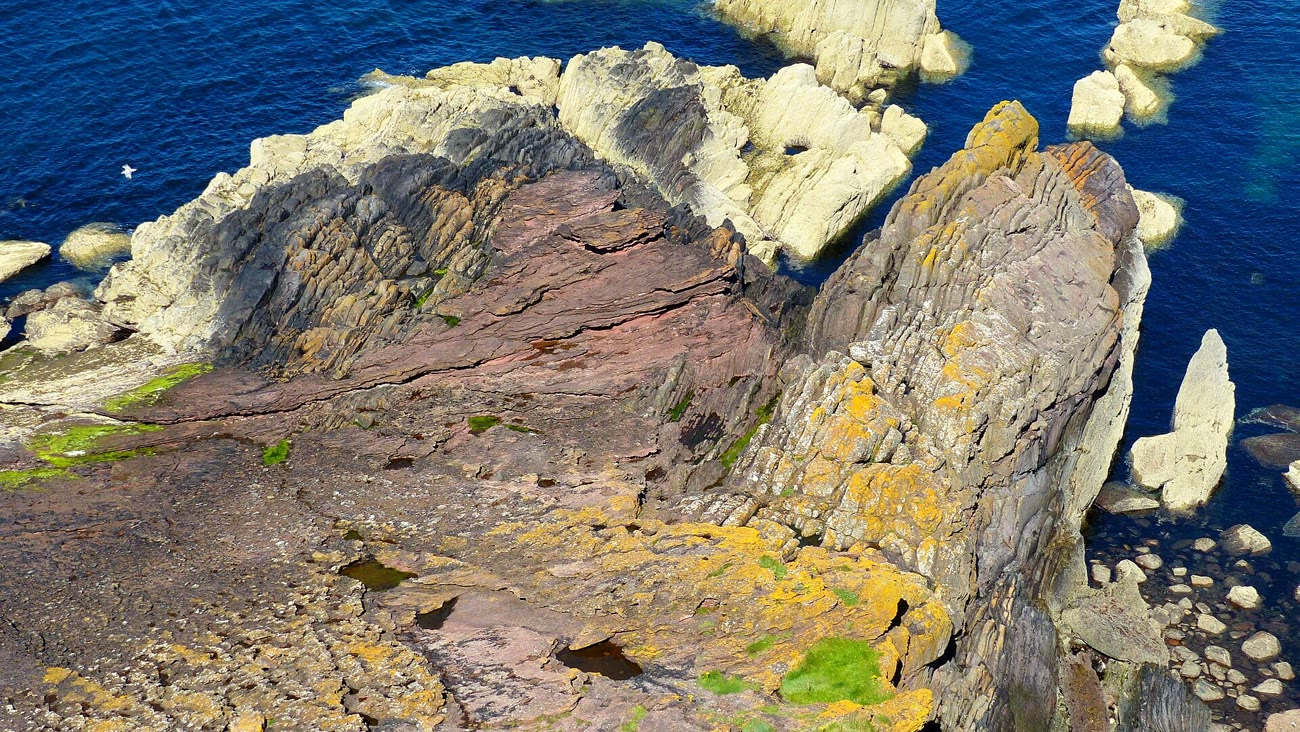
\includegraphics[width=0.7\linewidth]{images/book3/b1-siccar-point.jpg}

{\small \omterm{def:b1:cross-sections:unconformity}{Ketidakselarasan} Hutton di Siccar Point: lapisan Silur abu-abu yang hampir tegak di bawah, lapisan Devon merah yang miring landai di atas. Foto PawełS, CC BY-SA 4.0 (Wikimedia Commons).}
% ledger: commons:siccar-point
\end{center}
\end{history}

\begin{inthefield}[Geologi untuk terowongan]
\begin{minipage}[t]{0.6\linewidth}\vspace{0pt}
Sebelum sebuah terowongan dirancang, ahli geologi teknik membuat penampang sepanjang jalurnya dari \omterm{def:b1:geological-maps:geological-map}{peta geologi}, dari lubang bor yang dibor berjarak sepanjang rute, dan dari survei geofisika. Mereka memperkirakan setiap satuan yang akan dipotong terowongan, sesar yang akan dilintasinya, dan tempat air mungkin masuk. Selama pengeboran, ahli geologi kontraktor mencatat batuan yang tersingkap di muka kerja pada setiap kemajuan, membandingkannya dengan ramalan, dan memperbarui penampang; lubang uji yang dibor di depan mesin menguji tanah sebelum mesin mencapainya, terutama di dekat sesar yang diramalkan atau di batu gamping yang mungkin menyimpan rongga. Zona sesar berupa batuan yang remuk merupakan bahaya klasik, lebih-lebih bila batuan yang sama terdapat di kedua sisinya dan tidak ada yang di muka kerja memberi peringatan.
\end{minipage}\hfill
\begin{minipage}[t]{0.37\linewidth}\vspace{0pt}
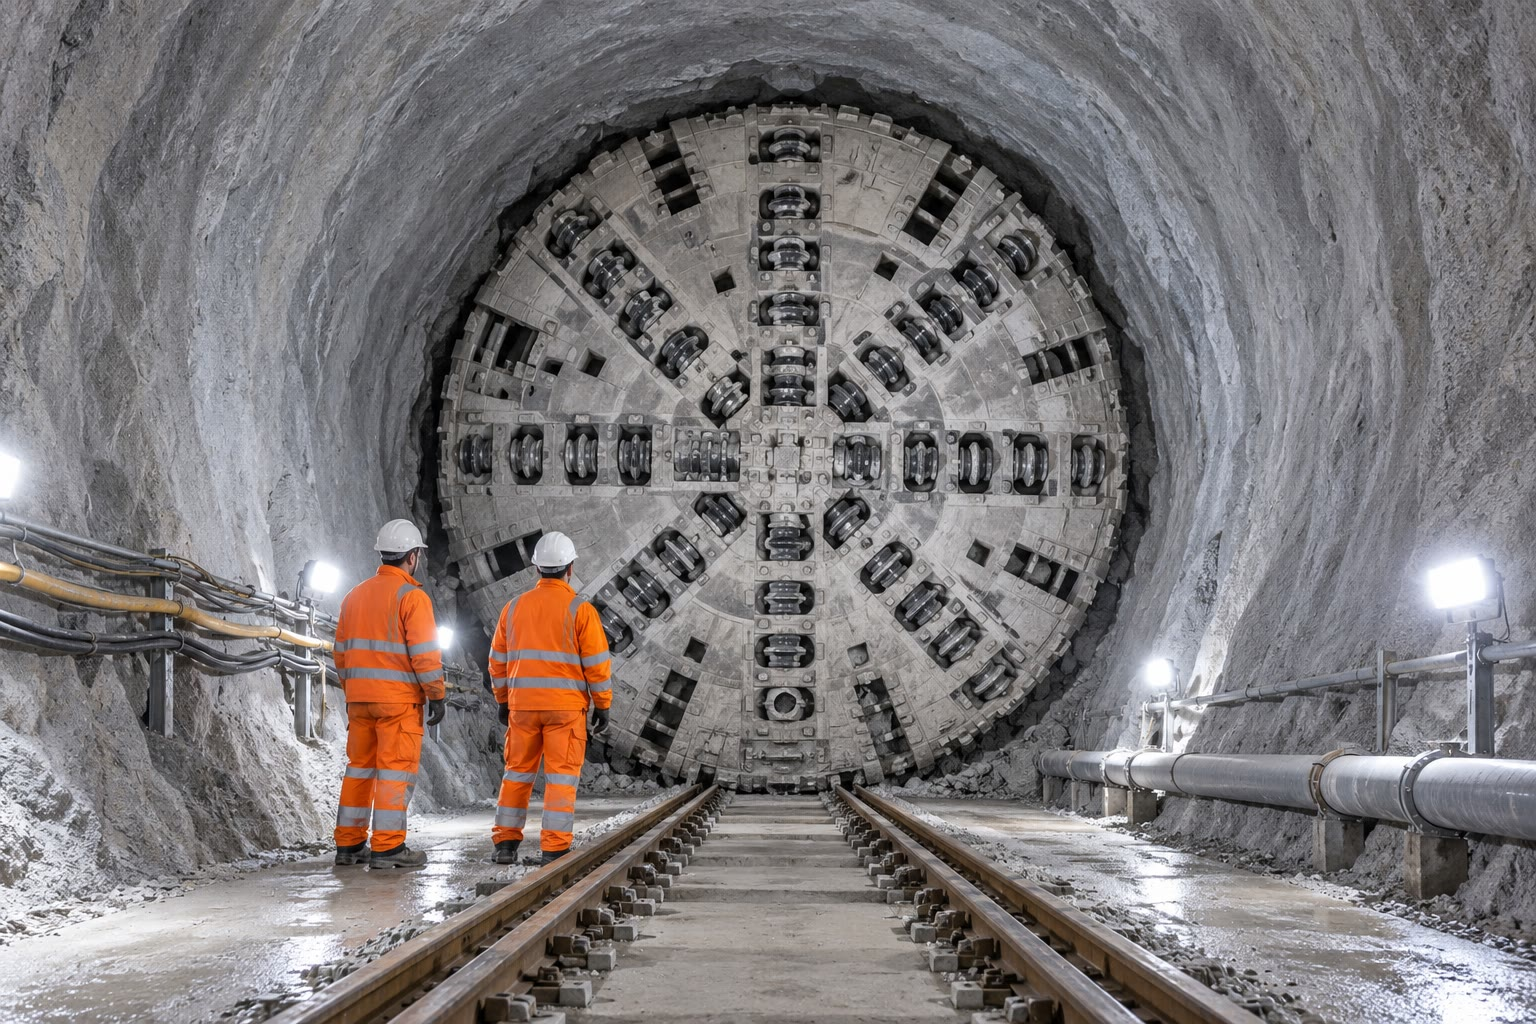
\includegraphics[width=\linewidth]{images/book3/ai/b1-tunnel-boring.jpg}
\end{minipage}
\end{inthefield}

\section{Latihan}

\begin{exercise}[$\star$]\label{exo:b1:cross-sections:1}
Sebuah penampang digambar dari peta pada skala 1:25\,000, dengan skala vertikal \qty{1}{cm} untuk \qty{100}{m}. Berapakah \omterm{def:b1:cross-sections:section}{eksagerasi vertikalnya}?
\end{exercise}

\begin{exercise}[$\star$]\label{exo:b1:cross-sections:2}
Sebuah lapisan miring \ang{40} ke arah \ang{090}. Berapakah \omterm{def:b1:cross-sections:apparent-dip}{kemiringan semunya} dalam penampang vertikal berazimut \ang{060}? Berazimut \ang{000}?
\end{exercise}

\begin{exercise}[$\star$]\label{exo:b1:cross-sections:3}
Sebuah lubang bor vertikal memotong \qty{120}{m} batu pasir yang perlapisannya miring \ang{12.16}. Berapakah \omterm{def:b1:cross-sections:thickness}{ketebalan sebenarnya} batu pasir itu?
\end{exercise}

\begin{exercise}[$\star$]\label{exo:b1:cross-sections:4}
Sebuah \omterm{def:b1:geological-maps:geological-map}{kontak} yang miring \ang{12} dalam bidang penampang digambar dengan \omterm{def:b1:cross-sections:section}{eksagerasi vertikal} 2, 3, dan 5. Pada sudut berapakah ia tampak?
\end{exercise}

\begin{exercise}[$\star\star$]\label{exo:b1:cross-sections:5}
Sebuah lapisan miring \ang{25}. \omterm{def:b1:geological-maps:geological-map}{Singkapannya} selebar \qty{300}{m}, diukur tegak lurus \omterm{def:b1:geological-maps:attitude}{jurus}. Hitunglah \omterm{def:b1:cross-sections:thickness}{ketebalan sebenarnya} (a) di tanah datar; (b) di tanah yang miring \ang{10} berlawanan dengan \omterm{def:b1:geological-maps:attitude}{arah kemiringan}, dengan lebar diukur sepanjang tanah; (c) di tanah yang miring \ang{10} searah dengan \omterm{def:b1:geological-maps:attitude}{kemiringan}.
\end{exercise}

\begin{exercise}[$\star\star$]\label{exo:b1:cross-sections:6}
Sebuah lapisan menunjukkan \omterm{def:b1:cross-sections:apparent-dip}{kemiringan semu} \ang{20} ke utara dalam penampang utara--selatan, dan \ang{30} ke timur dalam penampang timur--barat. Carilah \omterm{def:b1:geological-maps:attitude}{arah kemiringan} dan \omterm{def:b1:geological-maps:attitude}{kemiringan} sebenarnya.
\end{exercise}

\begin{exercise}[$\star\star$]\label{exo:b1:cross-sections:7}
Dasar batu gamping di sayap timur miring \ang{12.16}. Berapakah jarak horizontal \omterm{def:b1:cross-sections:structure-contour}{kontur struktur} yang digambar setiap \qty{100}{m}? Periksalah pada \omterm{def:b1:cross-sections:structure-contour}{peta kontur struktur}.
\end{exercise}

\begin{exercise}[$\star\star$]\label{exo:b1:cross-sections:8}
Dari tabel lubang bor, hitunglah elevasi dasar serpih di B1 dan B3. Di atas B2, serpih telah tererosi: dari \omterm{def:b1:cross-sections:thickness}{ketebalan vertikal} batu gamping, carilah elevasi dasar yang akan dimilikinya di sana, dan \omterm{def:b1:cross-sections:apparent-dip}{kemiringan semu} \omterm{def:b1:geological-maps:geological-map}{kontak} itu antara B1 dan B2 dalam penampang C--D. Apa yang dikatakan perbandingan B1 dan B3 tentang \omterm{def:b1:geological-maps:fold}{lipatannya}?
\end{exercise}

\begin{exercise}[$\star\star$]\label{exo:b1:cross-sections:9}
Sebuah sesar normal yang miring \ang{50} ke arah \ang{180} memiliki \omterm{def:b1:cross-sections:throw}{lompatan vertikal} \qty{150}{m}. Hitunglah \omterm{def:b1:cross-sections:throw}{lompatan horizontalnya}. Dalam penampang vertikal berazimut \ang{150}, berapakah \omterm{def:b1:cross-sections:apparent-dip}{kemiringan semu} sesar itu dan pemisahan kedua pemotongan sebuah lapisan horizontal sepanjang penampang?
\end{exercise}

\begin{exercise}[$\star\star\star$]\label{exo:b1:cross-sections:10}
Untuk sebuah lapisan yang miring \ang{40}, pada arah penampang yang mana \omterm{def:b1:cross-sections:apparent-dip}{kemiringan semunya} setengah dari \omterm{def:b1:geological-maps:attitude}{kemiringan} sebenarnya, yaitu \ang{20}? Tunjukkan bahwa \omterm{def:b1:cross-sections:apparent-dip}{kemiringan semu} berubah sedikit di dekat \omterm{def:b1:geological-maps:attitude}{arah kemiringan} dan cepat di dekat \omterm{def:b1:geological-maps:attitude}{jurus}.
\end{exercise}

\begin{exercise}[$\star\star\star$]\label{exo:b1:cross-sections:11}
Sebuah lubang bor memotong batu gamping sayap timur (\omterm{def:b1:cross-sections:thickness}{ketebalan sebenarnya} \qty{176.0}{m}, \omterm{def:b1:geological-maps:attitude}{kemiringan} \ang{12.16} ke arah \ang{080.7}). Berapa panjang inti yang diperoleh (a) bila vertikal; (b) bila miring \ang{60} di bawah horizontal ke arah \ang{260.7}; (c) miring \ang{60} ke arah \ang{080.7}? (Petunjuk: panjangnya adalah $t/\cos\psi$, dengan $\psi$ sudut antara lubang bor dan normal perlapisan.)
\end{exercise}

\begin{exercise}[$\star\star\star$]\label{exo:b1:cross-sections:12}
Pada \omterm{def:b1:cross-sections:unconformity}{ketidakselarasan sudut}, lapisan di bawah miring \ang{70} ke arah \ang{090} dan lapisan di atas miring \ang{20} ke arah \ang{270}, dengan \omterm{def:b1:geological-maps:attitude}{jurus} yang sama. Putarlah seluruh \omterm{def:b1:geological-maps:geological-map}{singkapan} terhadap \omterm{def:b1:geological-maps:attitude}{jurusnya} untuk membawa lapisan atas kembali mendatar: berapakah \omterm{def:b1:geological-maps:attitude}{kemiringan} lapisan bawah ketika lapisan atas diendapkan? Tuliskan sejarah \omterm{def:b1:geological-maps:geological-map}{singkapan} itu secara berurutan.
\end{exercise}

\section{Soal: Sebuah terowongan di bawah Perbukitan Varden}

\begin{problem}[{Soal akhir pekan --- batuan mana yang akan dipotong terowongan, di mana ia bertemu sesar, dan berapa banyak batu gamping yang akan dibor}]
\label{pb:b1:cross-sections:1}
% numbers from figdata/bachelor-1/varden_sections.py (model region.py) and the scratch calculator
Terowongan membentang tepat ke timur sepanjang garis C--D ($y = \qty{6}{km}$) pada elevasi tetap \qty{200}{m}, dari $x = \qty{1}{km}$ sampai $x =
\qty{9}{km}$. Elevasi tanah sepanjang C--D, setiap kilometer dari $x = 0$, adalah:
\begin{center}
\small
\begin{tabular}{lccccccccccc}
\hline
$x$ (km) & 0 & 1 & 2 & 3 & 4 & 5 & 6 & 7 & 8 & 9 & 10 \\
$z$ (m) & 509 & 556 & 467 & 370 & 435 & 534 & 501 & 455 & 406 & 339 & 405 \\
\hline
\end{tabular}
\end{center}
Gunakan tabel lubang bor bab ini, penampang C--D yang digambar dengan $e = 3$, orientasi sayap timur (\omterm{def:b1:geological-maps:attitude}{kemiringan} \ang{12.16} ke arah \ang{080.7}; sayap barat adalah bayangan cerminnya, miring ke arah \ang{279.3}), dan sesar normal, yang miring \ang{60} ke arah \ang{120}, memiliki \omterm{def:b1:cross-sections:throw}{lompatan vertikal} \qty{200}{m}, dan melintasi titik $x = \qty{4.30}{km}$, $y = \qty{1.00}{km}$, $z = \qty{250}{m}$.

\medskip
\noindent\textbf{Bagian I --- Profil dan satuan.}
\begin{enumerate}
  \item Berapakah ketebalan batuan terbesar dan terkecil di atas terowongan pada titik-titik kilometer antara $x = 1$ dan $x = 9$?
  \item Pada penampang yang tercetak, \qty{1}{km} jarak horizontal berukuran \qty{1.4}{cm} dan \qty{1}{km} elevasi berukuran \qty{4.2}{cm}. Periksalah bahwa $e = 3$.
  \item Dari log B2, carilah elevasi dasar batu pasir di puncak \omterm{def:b1:geological-maps:fold}{antiklin}.
  \item Dalam satuan apa terowongan berada pada $x = \qty{3.5}{km}$?
  \item Hitunglah elevasi dasar batu gamping di B1 dan B3.
  \item Dari penampang, daftarkan berurutan satuan-satuan yang dipotong terowongan dari $x = 1$ sampai $x = \qty{9}{km}$.
\end{enumerate}

\medskip
\noindent\textbf{Bagian II --- Kemiringan dalam penampang.}
\begin{enumerate}[resume]
  \item Hitunglah \omterm{def:b1:cross-sections:apparent-dip}{kemiringan semu} sayap timur dalam C--D dari orientasinya.
  \item Periksalah dari elevasi dasar batu gamping di B2 dan B3.
  \item Pada sudut berapakah sayap timur digambar dalam penampang dengan $e = 3$?
  \item Hitunglah \omterm{def:b1:cross-sections:apparent-dip}{kemiringan semu} sesar dalam C--D.
  \item Mengapa \omterm{def:b1:cross-sections:apparent-dip}{kemiringan semu} sayap-sayap dalam C--D begitu dekat dengan \omterm{def:b1:geological-maps:attitude}{kemiringan} sebenarnya mereka, dan \omterm{def:b1:geological-maps:attitude}{kemiringan} sesar kurang demikian?
\end{enumerate}

\medskip
\noindent\textbf{Bagian III --- Sesar.}
\begin{enumerate}[resume]
  \item Tunjukkan bahwa, pada bidang $y = \qty{6}{km}$, sesar berada pada
        \[ x = 4300 + \frac{2500 - (z - 250)\tan\ang{30}}{\sin\ang{120}}
           \quad\text{(meter)}. \]
  \item Di mana terowongan bertemu sesar?
  \item Hitunglah \omterm{def:b1:cross-sections:throw}{lompatan horizontal} sesar, dan pemisahan kedua pemotongan suatu \omterm{def:b1:geological-maps:geological-map}{kontak} sepanjang C--D.
  \item Blok mana yang turun, dan satuan mana yang berada pada tingkat terowongan di setiap sisi sesar?
  \item Mengapa sesar itu merupakan bahaya yang tidak dapat dilihat oleh regu penggali dari batuan di muka kerja? Bagaimana para insinyur mengantisipasinya?
\end{enumerate}

\medskip
\noindent\textbf{Bagian IV --- Batu gamping.}
\begin{enumerate}[resume]
  \item Berapakah \omterm{def:b1:cross-sections:thickness}{ketebalan vertikal} batu gamping di B1?
  \item Berapakah \omterm{def:b1:cross-sections:thickness}{ketebalan sebenarnya}?
  \item Tunjukkan bahwa, di barat sesar pada C--D, dasar batu pasir berada pada
        \[ z_b = 160.16 - |x - 3500|\tan\ang{12.0} \quad\text{(meter)}. \]
  \item Terowongan berada di dalam batu gamping bila dasarnya berada di bawah \qty{200}{m} dan puncaknya di atas. Tunjukkan bahwa ini terjadi untuk $377.1 < |x - 3500|
        < 1224.0$.
  \item Berikan empat titik tempat terowongan memasuki dan meninggalkan batu gamping.
  \item Tunjukkan bahwa panjang yang dibor pada setiap sayap adalah $h/\tan\beta$, dengan $h$ \omterm{def:b1:cross-sections:thickness}{ketebalan vertikal} dan $\beta$ \omterm{def:b1:cross-sections:apparent-dip}{kemiringan semu}, lalu hitunglah.
  \item Berapa panjang batu gamping total yang dilalui terowongan?
\end{enumerate}
\end{problem}
